\section{Design}

\subsection{System Architecture Diagrams}

\subsubsection{Component-Level Architecture}

The analog signal acquisition and conditioning system connects seven hardware components to the Arduino Mega 2560 microcontroller through four distinct interfaces: ADC (analog), OneWire (digital), I2C (LCD), and GPIO (LEDs). The component-level architecture diagram in \citeimg{fig:system_structural_diagram} illustrates the physical topology and communication protocols between all system elements.

The NTC thermistor connects through a voltage divider to analog pin A0, providing a continuously variable voltage that the 10-bit ADC samples at each acquisition cycle. The series resistor (10 k$\Omega$) and the NTC form a resistive divider whose midpoint voltage is inversely related to temperature, enabling the microcontroller to compute the thermistor resistance and, through the Steinhart-Hart Beta equation, the corresponding temperature in degrees Celsius. The DS18B20 connects through a single OneWire data line (with a 4.7 k$\Omega$ pull-up resistor) to digital pin 2, communicating temperature readings as digital data packets with 10-bit resolution. The LCD 1602 connects via the I2C bus (SDA on pin 20, SCL on pin 21), allowing the display to be updated with formatted temperature and status information. Three LEDs connect through 220 $\Omega$ current-limiting resistors to digital pins 8, 9, and 10, providing immediate visual feedback on system and alert conditions.

\begin{figure}[H]
\centering
\begin{tikzpicture}[
    comp/.style={draw, rectangle, rounded corners, minimum width=3.5cm,
                 minimum height=1.0cm, text centered, align=center, fill=blue!10},
    mcu/.style={draw, rectangle, rounded corners, minimum width=4.0cm,
                minimum height=1.2cm, text centered, align=center, fill=green!15, line width=1.2pt},
    conn/.style={->, thick, >=Stealth}]

    % MCU at center
    \node[mcu] (mcu) at (0, 0) {Arduino Mega 2560\\ATmega2560};

    % Sensors on the left
    \node[comp, fill=red!10] (ntc) at (-6.5, 2.0) {NTC Thermistor\\10K, $\beta$=3950};
    \node[comp, fill=red!10] (ds)  at (-6.5, -2.0) {DS18B20\\Digital Temp};

    % Display on the right top
    \node[comp, fill=yellow!15] (lcd) at (6.5, 2.0) {LCD 1602\\I2C Display};

    % LEDs on the right bottom
    \node[comp, fill=green!15] (ledg) at (5.0, -1.5) {Green LED\\(Normal)};
    \node[comp, fill=red!15]   (ledr) at (5.0, -2.8) {Red LED\\(Analog Alert)};
    \node[comp, fill=orange!15](ledy) at (5.0, -4.1) {Yellow LED\\(Digital Alert)};

    % Serial out bottom
    \node[comp, fill=gray!15] (uart) at (0, -4.5) {Serial Terminal\\(STDIO via UART)};

    % Connections
    \draw[conn, orange] (ntc.east) -- node[above, font=\scriptsize]{ADC (A0)} (mcu.west |- ntc);
    \draw[conn, blue]   (ds.east)  -- node[below, font=\scriptsize]{OneWire (D2)} (mcu.west |- ds);
    \draw[conn, green!60!black] (mcu.east |- lcd) -- node[above, font=\scriptsize]{I2C (SDA/SCL)} (lcd.west);
    \draw[conn] (mcu.east |- ledg) -- node[above, font=\scriptsize]{GPIO D8} (ledg.west);
    \draw[conn] (mcu.east |- ledr) -- node[above, font=\scriptsize]{GPIO D9} (ledr.west);
    \draw[conn] (mcu.east |- ledy) -- node[above, font=\scriptsize]{GPIO D10} (ledy.west);
    \draw[conn, <->] (mcu.south) -- node[right, font=\scriptsize]{UART 9600} (uart.north);
\end{tikzpicture}
\caption{System structural diagram --- component-level architecture}
\label{fig:system_structural_diagram}
\end{figure}

The data flows in the system follow distinct paths. Sensor data flows inward from the NTC thermistor and DS18B20 into the microcontroller, where it is processed by the acquisition task, then conditioned through a three-stage pipeline (saturation, median filter, EWMA) before being evaluated by the threshold alert FSM. Processed results flow outward through two channels: the I2C bus to the LCD for real-time display of conditioned values, and the UART serial port for detailed STDIO reports showing raw, median-filtered, and EWMA values at each pipeline stage.

\subsubsection{Layered Software Architecture}

The software architecture follows a layered design pattern that separates hardware-specific drivers from application logic, enabling code reuse across laboratory projects and simplifying maintenance. Compared to Lab 3.1, the service layer now includes the SignalConditioner module, which implements the three-stage conditioning pipeline that is the central contribution of this lab. \citeimg{fig:layered_architecture} illustrates the five-layer hierarchy used in this system.

\begin{figure}[H]
\centering
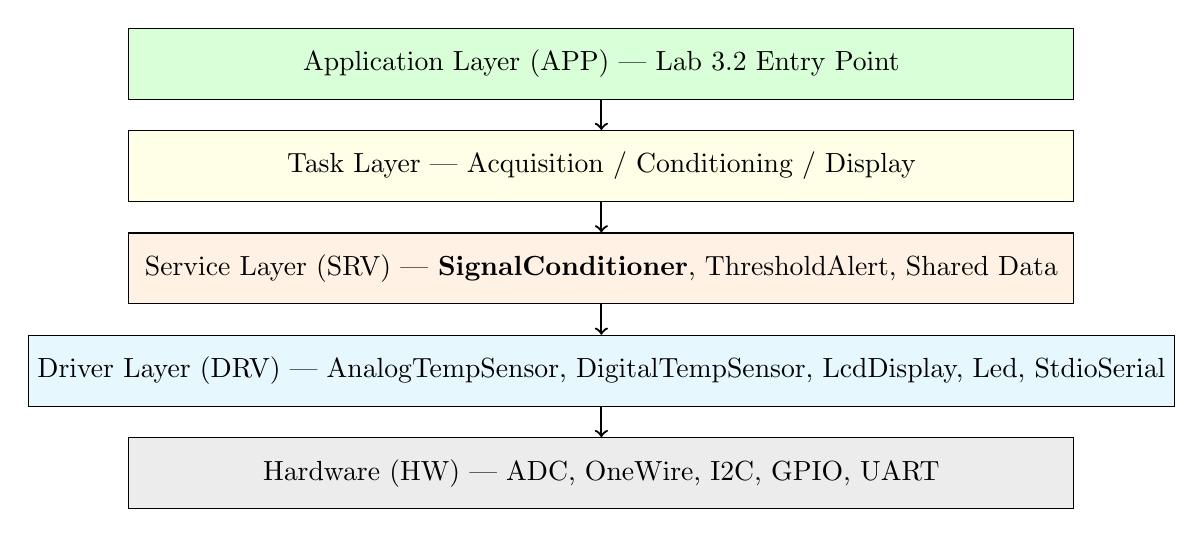
\begin{tikzpicture}[
    box/.style={draw, rectangle, minimum width=12cm, minimum height=0.9cm,
                text centered, align=center, fill=blue!10},
    node distance=0.4cm]
    \node[box, fill=green!15]  (app)  at (0, 0)    {Application Layer (APP) --- Lab 3.2 Entry Point};
    \node[box, fill=yellow!10] (task) at (0, -1.3)  {Task Layer --- Acquisition / Conditioning / Display};
    \node[box, fill=orange!10] (srv)  at (0, -2.6)  {Service Layer (SRV) --- \textbf{SignalConditioner}, ThresholdAlert, Shared Data};
    \node[box, fill=cyan!10]   (drv)  at (0, -3.9)  {Driver Layer (DRV) --- AnalogTempSensor, DigitalTempSensor, LcdDisplay, Led, StdioSerial};
    \node[box, fill=gray!15]   (hw)   at (0, -5.2)  {Hardware (HW) --- ADC, OneWire, I2C, GPIO, UART};
    \foreach \a/\b in {app/task, task/srv, srv/drv, drv/hw}
        \draw[->, thick] (\a) -- (\b);
\end{tikzpicture}
\caption{Layered software architecture of the signal conditioning system}
\label{fig:layered_architecture}
\end{figure}

The Hardware Layer (HW) encompasses the physical peripherals: the ADC for the NTC thermistor, the OneWire bus for the DS18B20, the I2C bus for the LCD, GPIO pins for the LEDs, and the UART for serial communication. The Driver Layer (DRV) contains reusable library modules that abstract hardware access behind clean C++ interfaces. The Service Layer (SRV) provides application-independent processing logic, including the new SignalConditioner module (saturation, median filter, EWMA), the ThresholdAlert module for hysteresis-based alert detection, and the shared data structures with their synchronization primitives. The Task Layer defines the three FreeRTOS tasks that implement the monitoring pipeline. The Application Layer (APP) is the lab entry point that initializes hardware, creates synchronization primitives, spawns tasks, and starts the FreeRTOS scheduler.

Each layer communicates only with its immediate neighbor, ensuring that application code never directly manipulates hardware registers, and driver modules can be tested and reused independently of the specific application logic.

\subsubsection{FreeRTOS Task Architecture}

The three FreeRTOS tasks operate as a pipeline, with well-defined data flows and synchronization points. Unlike Lab 3.1 where Task 2 applied only threshold alerting, in Lab 3.2 Task 2 additionally runs each raw sensor reading through the SignalConditioner pipeline before feeding the conditioned value to the ThresholdAlert FSM. \citeimg{fig:task_architecture} shows the task communication topology.

\begin{figure}[H]
\centering
\begin{tikzpicture}[
    task/.style={draw, rectangle, rounded corners, minimum width=3.8cm,
                 minimum height=1.5cm, text centered, align=center, fill=blue!10, line width=1pt},
    data/.style={draw, rectangle, minimum width=2.5cm, minimum height=0.8cm,
                 text centered, align=center, fill=yellow!15, font=\small},
    sync/.style={draw, ellipse, minimum width=2.0cm, minimum height=0.7cm,
                 text centered, align=center, fill=orange!15, font=\small},
    arr/.style={->, thick, >=Stealth}]

    % Tasks
    \node[task] (t1) at (0, 0)    {Task 1\\\textbf{Acquisition}\\50 ms, Prio 3};
    \node[task] (t2) at (6, 0)    {Task 2\\\textbf{Conditioning}\\Event, Prio 2};
    \node[task] (t3) at (12, 0)   {Task 3\\\textbf{Display}\\500 ms, Prio 1};

    % Shared data
    \node[data] (sd) at (3, -2.5) {g\_sensorData};
    \node[data] (ad) at (9, -2.5) {g\_alertData};

    % Sync primitives
    \node[sync] (sem) at (3, 1.8) {Semaphore};
    \node[sync] (mtx) at (6, -4.0) {Mutex};

    % Arrows
    \draw[arr, blue] (t1) -- node[above, font=\scriptsize]{give} (sem);
    \draw[arr, blue] (sem) -- node[above, font=\scriptsize]{take} (t2);
    \draw[arr, red]  (t1.south) -- node[left, font=\scriptsize]{write raw} (sd.north west);
    \draw[arr, red]  (sd.north east) -- node[right, font=\scriptsize]{read raw} (t2.south);
    \draw[arr, purple] (t2.south) -- node[left, font=\scriptsize]{write cond.} (sd.north east);
    \draw[arr, red]  (t2.south) -- node[left, font=\scriptsize]{write} (ad.north west);
    \draw[arr, red]  (ad.north east) -- node[right, font=\scriptsize]{read} (t3.south);
    \draw[arr, dashed] (mtx) -- (sd);
    \draw[arr, dashed] (mtx) -- (ad);
\end{tikzpicture}
\caption{FreeRTOS task communication architecture}
\label{fig:task_architecture}
\end{figure}

Task 1 (Acquisition) runs at the highest priority (3) with a 50 ms period using \texttt{vTaskDelayUntil()} for drift-free timing. It reads both sensors, writes the raw results to \texttt{g\_sensorData} under mutex protection, and gives the binary semaphore to notify Task 2. Task 2 (Conditioning) runs at medium priority (2) and blocks on the semaphore until new data is available, then reads the raw sensor data, applies the SignalConditioner pipeline (saturation, median filter, EWMA) independently for each sensor, feeds the conditioned values to the ThresholdAlert FSM, writes both the conditioned readings and alert status back to the shared structures under mutex protection, and updates the LED indicators. Task 3 (Display) runs at the lowest priority (1) with a 500 ms period, reading both shared data structures under mutex protection and formatting the output for the LCD and STDIO, now including raw, median-filtered, and EWMA values for each sensor.

\subsubsection{Signal Conditioning Pipeline}

The signal conditioning pipeline is the central contribution of Lab 3.2. It processes each raw temperature reading through three sequential stages, progressively removing noise and producing a stable, reliable signal for threshold evaluation. \citeimg{fig:pipeline_flowchart} illustrates the complete pipeline as implemented by \texttt{SignalConditioner::process()}.

\tikzset{
    startstop/.style={rectangle, rounded corners, minimum width=2.5cm,
        minimum height=0.7cm, text centered, align=center, draw=black, fill=gray!15},
    process/.style={rectangle, minimum width=2.5cm,
        minimum height=0.7cm, text centered, align=center, draw=black, fill=blue!10},
    decision/.style={diamond, aspect=2.5, minimum width=2cm,
        minimum height=0.7cm, text centered, align=center, draw=black, fill=orange!15},
    io/.style={trapezium, trapezium left angle=70, trapezium right angle=110,
        minimum width=2.5cm, minimum height=0.7cm, text centered, align=center,
        draw=black, fill=green!10},
    arrow/.style={thick,->,>=Stealth}
}

\begin{figure}[H]
\centering
\begin{tikzpicture}
    \node (start)  [startstop] at (0,    0.0)  {Start: process(raw)};
    \node (store)  [process]   at (0,   -1.8)  {Store raw value\\(\texttt{\_lastRaw = raw})};
    \node (nanck)  [decision]  at (0,   -4.3)  {raw is\\NaN?};
    \node (nanrep) [process]   at (5.5, -4.3)  {Replace with\\midpoint of range};
    \node (satur)  [process]   at (0,   -6.8)  {Saturate: clamp\\to [min, max]};
    \node (insert) [process]   at (0,   -8.6)  {Insert saturated value\\into circular buffer};
    \node (median) [process]   at (0,  -10.4)  {Copy buffer, insertion\\sort, select median};
    \node (ewchk)  [decision]  at (0,  -13.0)  {EWMA\\initialized?};
    \node (seed)   [process]   at (5.5,-13.0)  {Seed EWMA with\\first median value};
    \node (ewma)   [process]   at (0,  -15.5)  {EWMA: $\alpha \cdot \mathrm{median}$\\$+ (1-\alpha) \cdot \mathrm{prev}$};
    \node (ret)    [startstop] at (0,  -17.3)  {Return EWMA value};

    \draw [arrow] (start)  -- (store);
    \draw [arrow] (store)  -- (nanck);
    \draw [arrow] (nanck)  -- node[above, font=\scriptsize]{Yes} (nanrep);
    \draw [arrow] (nanck)  -- node[right, font=\scriptsize]{No}  (satur);
    \draw [arrow] (nanrep.south) -- (5.5, -6.8) -- (satur);
    \draw [arrow] (satur)  -- (insert);
    \draw [arrow] (insert) -- (median);
    \draw [arrow] (median) -- (ewchk);
    \draw [arrow] (ewchk)  -- node[above, font=\scriptsize]{No} (seed);
    \draw [arrow] (ewchk)  -- node[right, font=\scriptsize]{Yes} (ewma);
    \draw [arrow] (seed.south) -- (5.5, -15.5) -- (ewma);
    \draw [arrow] (ewma)   -- (ret);
\end{tikzpicture}
\caption{Signal conditioning pipeline flowchart (\texttt{SignalConditioner::process()})}
\label{fig:pipeline_flowchart}
\end{figure}

The first stage, saturation, clamps the raw reading to a physically valid range (default $-40$\textdegree C to $+125$\textdegree C), rejecting readings that fall outside the sensor's operating envelope. If the raw input is NaN (indicating a sensor communication failure), the saturator substitutes the midpoint of the valid range, preventing NaN from propagating through the pipeline and corrupting the median buffer and EWMA accumulator. The second stage, the median filter, maintains a fixed-size circular buffer (configurable up to 9 samples) and computes the median of the current window contents by copying the buffer, sorting the copy via insertion sort, and selecting the middle element. The median filter is particularly effective at removing impulsive noise ("salt and pepper" spikes) caused by electrical interference or transient sensor glitches, without introducing the phase lag inherent in linear averaging filters. The third stage, the exponentially weighted moving average (EWMA), applies a first-order IIR filter with configurable smoothing factor $\alpha$: $y_n = \alpha \cdot x_n + (1-\alpha) \cdot y_{n-1}$, where $x_n$ is the median-filtered value and $y_{n-1}$ is the previous EWMA output. Lower $\alpha$ values produce smoother output with more lag, while higher values track rapid changes more closely at the cost of less noise suppression.

\subsection{Hardware Configuration}

\subsubsection{Electrical Schematic Description}

The circuit for Lab 3.2 uses the same hardware configuration as Lab 3.1, since the signal conditioning improvements are entirely software-based. The NTC thermistor and its 10 k$\Omega$ series resistor form a voltage divider between the 5V supply rail and ground, with the midpoint connected to analog pin A0. At the nominal temperature of 25\textdegree C, the NTC resistance equals the series resistance, producing approximately 2.5V at the midpoint. As temperature increases, the NTC resistance decreases, pulling the midpoint voltage higher; the ADC converts this voltage to a 10-bit digital value (0--1023), from which the firmware computes resistance and then temperature using the Beta parameter equation.

The DS18B20 requires a 4.7 k$\Omega$ pull-up resistor on its data line (pin D2) because the OneWire protocol uses an open-drain bus topology. The sensor is powered from the 5V rail (not operating in parasitic power mode), and communicates using precisely timed pulse sequences. Each LED is driven through a 220 $\Omega$ current-limiting resistor, restricting the forward current to approximately 15 mA at the GPIO output voltage of 5V, well within the safe operating limits for both the LEDs and the ATmega2560 GPIO pins. The I2C LCD module includes an onboard PCF8574 I/O expander at address 0x27, which handles the parallel data interface to the HD44780 controller; the microcontroller communicates with it over just two wires (SDA and SCL).

\begin{figure}[H]
\centering
\begin{circuitikz}[scale=0.85, transform shape]
    % Title area
    \node[font=\bfseries] at (5, 1.5) {Arduino Mega 2560 --- Dual Sensor with Signal Conditioning};

    % NTC Thermistor voltage divider
    \draw (0, 0) node[anchor=east, font=\small]{5V}
        to[R, l=$10\,\mathrm{k}\Omega$, a=Series] (3, 0)
        to[short] (4.5, 0)
        node[anchor=west, font=\small]{A0};
    \draw (3, 0) to[short] (3, -1.5)
        to[thR, l_=NTC, a=10k] (3, -3.5)
        node[ground]{};
    \node[font=\scriptsize, anchor=west] at (4.5, -0.5) {(Analog Input)};

    % DS18B20
    \draw (0, -5) node[anchor=east, font=\small]{5V}
        to[R, l=$4.7\,\mathrm{k}\Omega$, a=Pull-up] (3, -5)
        to[short] (4.5, -5)
        node[anchor=west, font=\small]{D2 (OneWire)};
    \draw (3, -5) to[short] (3, -6)
        to[short] (1.5, -6)
        node[anchor=east, font=\small, align=right]{DS18B20\\DQ};
    \draw (1.5, -6.8) node[anchor=east, font=\small]{VCC} to[short] (3, -6.8)
        to[short] (3, -6.8) node[anchor=west, font=\small]{5V};
    \draw (1.5, -7.5) node[anchor=east, font=\small]{GND}
        to[short] (3, -7.5) node[ground]{};

    % I2C LCD
    \draw (7, 0) node[anchor=west, font=\small]{SDA (D20)}
        to[short] (10, 0)
        node[anchor=west, font=\small]{LCD SDA};
    \draw (7, -1) node[anchor=west, font=\small]{SCL (D21)}
        to[short] (10, -1)
        node[anchor=west, font=\small]{LCD SCL};
    \node[font=\scriptsize] at (10.5, -2) {LCD 1602 I2C};
    \node[font=\scriptsize] at (10.5, -2.5) {Addr: 0x27};

    % Green LED
    \draw (7, -4) node[anchor=west, font=\small]{D8}
        to[R, l=$220\,\Omega$] (9.5, -4)
        to[leD*, color=green] (11.5, -4)
        node[ground]{};
    \node[font=\scriptsize, green!60!black] at (11.5, -3.5) {GREEN};

    % Red LED
    \draw (7, -5.5) node[anchor=west, font=\small]{D9}
        to[R, l=$220\,\Omega$] (9.5, -5.5)
        to[leD*, color=red] (11.5, -5.5)
        node[ground]{};
    \node[font=\scriptsize, red] at (11.5, -5.0) {RED};

    % Yellow LED
    \draw (7, -7) node[anchor=west, font=\small]{D10}
        to[R, l=$220\,\Omega$] (9.5, -7)
        to[leD*, color=yellow!80!black] (11.5, -7)
        node[ground]{};
    \node[font=\scriptsize, orange] at (11.5, -6.5) {YELLOW};
\end{circuitikz}
\caption{Complete circuit schematic of the dual-sensor system with signal conditioning}
\label{fig:circuit_schematic}
\end{figure}

\subsubsection{Wokwi Circuit Configuration}

The Wokwi simulation configuration file defines the virtual firmware path and debug symbols for Lab 3.2:

\begin{lstlisting}[language=json, caption=Wokwi configuration file (wokwi.toml), label=lst:wokwi_config]
[wokwi]
version = 1
firmware = "../../.pio/build/lab3_2/firmware.hex"
elf = "../../.pio/build/lab3_2/firmware.elf"
\end{lstlisting}

\begin{figure}[H]
\centering
\IfFileExists{resources/Design/ElectricalSchematics/wokwi_circuit.png}{%
    
\includegraphics[width=0.85\textwidth]{resources/Design/ElectricalSchematics/wokwi_circuit.png}%
}{%
    \fbox{\parbox{0.83\textwidth}{\centering\color{gray}\small
        [Screenshot pending --- run the Wokwi simulation and save to\\
        resources/Design/ElectricalSchematics/wokwi\_circuit.png]}}%
}
\caption{Wokwi simulation circuit (active run)}
\label{fig:wokwi_circuit}
\end{figure}

\subsection{Project Structure and Modules}

The project follows the established repository convention, with lab-specific code in a dedicated folder and reusable libraries shared across labs. Compared to Lab 3.1, the key structural addition is the \texttt{SignalConditioner} library module, which implements the saturation, median filter, and EWMA pipeline as a reusable, configurable C++ class.

\begin{lstlisting}[caption=Project directory structure for Lab 3.2, label=lst:project_structure]
labs/
|-- platformio.ini
|-- src/
|   |-- main.cpp                    (Lab selector entry point)
|-- lab/
|   |-- lab3_2/
|       |-- lab3_2_main.cpp         (Lab entry point)
|       |-- lab3_2_main.h           (Lab entry point header)
|       |-- sensor_data.h           (Shared data + sync primitives)
|       |-- sensor_data.cpp         (Shared data definitions)
|       |-- task_acquisition.h      (Task 1 interface)
|       |-- task_acquisition.cpp    (Task 1 implementation)
|       |-- task_conditioning.h     (Task 2 interface)
|       |-- task_conditioning.cpp   (Task 2 implementation)
|       |-- task_display.h          (Task 3 interface)
|       |-- task_display.cpp        (Task 3 implementation)
|-- lib/
|   |-- SignalConditioner/          (NEW -- saturation + median + EWMA)
|   |   |-- SignalConditioner.h
|   |   |-- SignalConditioner.cpp
|   |-- AnalogTempSensor/           (NTC thermistor driver)
|   |   |-- AnalogTempSensor.h
|   |   |-- AnalogTempSensor.cpp
|   |-- DigitalTempSensor/          (DS18B20 OneWire driver)
|   |   |-- DigitalTempSensor.h
|   |   |-- DigitalTempSensor.cpp
|   |-- ThresholdAlert/             (Hysteresis + debounce FSM)
|   |   |-- ThresholdAlert.h
|   |   |-- ThresholdAlert.cpp
|   |-- LcdDisplay/                 (I2C LCD driver, reused)
|   |   |-- LcdDisplay.h
|   |   |-- LcdDisplay.cpp
|   |-- Led/                        (LED driver, reused)
|   |   |-- Led.h
|   |   |-- Led.cpp
|   |-- StdioSerial/                (STDIO redirection, reused)
|       |-- StdioSerial.h
|       |-- StdioSerial.cpp
|-- wokwi/
    |-- lab3.2/
        |-- diagram.json            (Wokwi circuit definition)
        |-- wokwi.toml              (Wokwi firmware path)
\end{lstlisting}

This structure reflects the layered architecture: reusable driver-layer and service-layer modules reside in \texttt{lib/}, while lab-specific task and application code resides in \texttt{lab/lab3\_2/}. The SignalConditioner module is designed as a standalone library so that it can be reused in future labs or applied to entirely different sensor types without modification. The separation ensures that sensor drivers, the threshold alert module, and now the signal conditioning pipeline can all evolve independently.

\subsection{Modular Implementation}

\subsubsection{SignalConditioner Module}

The SignalConditioner module is the new contribution of Lab 3.2. It encapsulates a configurable three-stage signal conditioning pipeline behind a simple \texttt{process()} interface: the caller provides a raw sensor reading and receives a fully conditioned output value. All intermediate values (saturated, median-filtered, EWMA) are stored internally and accessible via getter methods, enabling the display task to report each pipeline stage for diagnostic purposes.

\begin{lstlisting}[language=C++, caption=SignalConditioner interface (SignalConditioner.h), label=lst:signal_conditioner_h]
class SignalConditioner {
public:
    SignalConditioner(uint8_t medianWindowSize,
                      float ewmaAlpha,
                      float minClamp, float maxClamp);
    float process(float rawValue);

    float getLastRaw() const;
    float getLastSaturated() const;
    float getLastMedian() const;
    float getLastEwma() const;

    uint8_t getWindowSize() const;
    float getAlpha() const;
    float getMinClamp() const;
    float getMaxClamp() const;

    bool isValid() const;
    uint8_t getSampleCount() const;
    void reset();

private:
    static const uint8_t MAX_WINDOW_SIZE = 9;
    float   _window[MAX_WINDOW_SIZE];
    uint8_t _windowSize, _count, _index;
    float   _ewmaAlpha, _ewmaValue;
    bool    _ewmaInitialized;
    float   _minClamp, _maxClamp;
    float   _lastRaw, _lastSaturated;
    float   _lastMedian, _lastEwma;

    float saturate(float value) const;
    float computeMedian() const;
};
\end{lstlisting}

The constructor accepts four parameters that fully configure the pipeline: the median window size (must be odd, clamped to the compile-time constant \texttt{MAX\_WINDOW\_SIZE} = 9), the EWMA smoothing factor $\alpha$ (0.0--1.0), and the saturation bounds. The fixed-size circular buffer avoids any dynamic memory allocation, which is critical on the ATmega2560 where heap fragmentation can lead to unpredictable failures. The \texttt{isValid()} method returns \texttt{true} only after the median window has been completely filled with samples, signaling to the caller that the output has stabilized.

The \texttt{process()} method is the core of the module. It executes the three stages in sequence: saturation clamping (with NaN replacement), insertion into the circular buffer followed by median computation, and EWMA filtering. On the first call, the EWMA accumulator is seeded with the median value rather than zero, avoiding an initial transient that would otherwise take several samples to decay.

\begin{lstlisting}[language=C++, caption=SignalConditioner::process() --- full pipeline implementation, label=lst:signal_conditioner_process]
float SignalConditioner::process(float rawValue) {
    _lastRaw = rawValue;

    // Stage 1: Saturation (NaN handled specially)
    float saturated;
    if (isnan(rawValue)) {
        saturated = (_minClamp + _maxClamp) / 2.0f;
    } else {
        saturated = saturate(rawValue);
    }
    _lastSaturated = saturated;

    // Stage 2: Median filter (circular buffer + sort)
    _window[_index] = saturated;
    _index = (_index + 1) % _windowSize;
    if (_count < _windowSize) { _count++; }
    _lastMedian = computeMedian();

    // Stage 3: EWMA
    if (!_ewmaInitialized) {
        _ewmaValue = _lastMedian;
        _ewmaInitialized = true;
    } else {
        _ewmaValue = _ewmaAlpha * _lastMedian
                   + (1.0f - _ewmaAlpha) * _ewmaValue;
    }
    _lastEwma = _ewmaValue;
    return _lastEwma;
}
\end{lstlisting}

The median computation uses insertion sort on a local copy of the active portion of the circular buffer. Although insertion sort has $O(n^2)$ worst-case complexity, with $n \leq 9$ the actual execution time is negligible (fewer than 81 comparisons in the worst case). The algorithm copies only the active elements (\texttt{\_count}, not \texttt{MAX\_WINDOW\_SIZE}), sorts the copy in ascending order, and returns the middle element. For windows with an even number of elements (only during the initial fill phase), it returns the lower-middle value.

\begin{lstlisting}[language=C++, caption=Median computation via insertion sort, label=lst:compute_median]
float SignalConditioner::computeMedian() const {
    float sorted[MAX_WINDOW_SIZE];
    uint8_t n = _count;
    for (uint8_t i = 0; i < n; i++) {
        sorted[i] = _window[i];
    }
    // Insertion sort
    for (uint8_t i = 1; i < n; i++) {
        float key = sorted[i];
        int8_t j = i - 1;
        while (j >= 0 && sorted[j] > key) {
            sorted[j + 1] = sorted[j];
            j--;
        }
        sorted[j + 1] = key;
    }
    return sorted[n / 2];
}
\end{lstlisting}

\begin{figure}[H]
\centering
\begin{tikzpicture}
    \node (start) [startstop] at (0,   0.0)  {computeMedian()};
    \node (copy)  [process]   at (0,  -1.8)  {Copy active elements\\to local array};
    \node (sort)  [process]   at (0,  -3.6)  {Insertion sort\\ascending order};
    \node (sel)   [process]   at (0,  -5.4)  {Select middle\\element: sorted[n/2]};
    \node (ret)   [startstop] at (0,  -7.2)  {Return median};

    \draw [arrow] (start) -- (copy);
    \draw [arrow] (copy)  -- (sort);
    \draw [arrow] (sort)  -- (sel);
    \draw [arrow] (sel)   -- (ret);
\end{tikzpicture}
\caption{Flowchart: SignalConditioner::computeMedian()}
\label{fig:flowchart_compute_median}
\end{figure}

\subsubsection{Sensor Acquisition Module (Task 1)}

The acquisition task reads both temperature sensors at a fixed 50 ms interval and publishes raw values to the shared data structure. It uses \texttt{vTaskDelayUntil()} for drift-free periodic execution. The DS18B20 employs a non-blocking read strategy: each cycle reads the result of the previous conversion and starts a new one, overlapping the 187.5 ms conversion time (at 10-bit resolution) with multiple sleep periods. \citeimg{fig:flowchart_acquisition} shows the task control flow.

\begin{figure}[H]
\centering
\begin{tikzpicture}
    \node (start) [startstop] at (0,    0.0)  {Task Start};
    \node (init)  [process]   at (0,   -1.8)  {Initialize NTC\\and DS18B20 sensors};
    \node (req1)  [process]   at (0,   -3.6)  {Request first\\DS18B20 conversion};
    \node (wait)  [process]   at (0,   -5.6)  {vTaskDelayUntil\\(50 ms period)};
    \node (adc)   [process]   at (0,   -7.4)  {Read NTC via ADC\\Convert to \textdegree C};
    \node (dchk)  [decision]  at (0,  -10.0)  {DS18B20\\conversion\\complete?};
    \node (dread) [process]   at (5.5, -10.0) {Read DS18B20\\temperature};
    \node (dlast) [process]   at (-5.5,-10.0) {Use last known\\temperature};
    \node (dreq)  [process]   at (0,  -12.5)  {Request next\\DS18B20 conversion};
    \node (mtx)   [process]   at (0,  -14.3)  {Mutex: write raw\\to g\_sensorData};
    \node (sem)   [process]   at (0,  -16.1)  {Give semaphore\\to Task 2};

    \draw [arrow] (start) -- (init);
    \draw [arrow] (init)  -- (req1);
    \draw [arrow] (req1)  -- (wait);
    \draw [arrow] (wait)  -- (adc);
    \draw [arrow] (adc)   -- (dchk);
    \draw [arrow] (dchk)  -- node[above, font=\scriptsize]{Yes} (dread);
    \draw [arrow] (dchk)  -- node[above, font=\scriptsize]{No}  (dlast);
    \draw [arrow] (dread.south) -- (5.5, -12.5) -- (dreq);
    \draw [arrow] (dlast.south) -- (-5.5, -12.5) -- (dreq);
    \draw [arrow] (dreq)  -- (mtx);
    \draw [arrow] (mtx)   -- (sem);
    \draw [arrow] (sem.west) -- ++(-3.0, 0) |- (wait.west);
\end{tikzpicture}
\caption{Sensor acquisition task flowchart (Task 1)}
\label{fig:flowchart_acquisition}
\end{figure}

The acquisition task writes only raw sensor values to \texttt{g\_sensorData}. It does not perform any signal conditioning --- that responsibility belongs exclusively to Task 2. This separation of concerns ensures that the acquisition timing is not affected by the computational cost of the conditioning pipeline, and allows the pipeline parameters to be modified independently of the sensor reading logic.

\subsubsection{Signal Conditioning Module (Task 2)}

The conditioning task is the core processing stage of the Lab 3.2 pipeline. It blocks on the binary semaphore until notified by Task 1, reads the raw temperature values from shared data, applies the SignalConditioner pipeline independently for each sensor channel, feeds the conditioned values to the ThresholdAlert FSM, and updates both the shared data structures and the LED indicators. \citeimg{fig:flowchart_conditioning} shows the complete task flow.

\begin{figure}[H]
\centering
\begin{tikzpicture}
    \node (start)  [startstop] at (0,    0.0)  {Task Start};
    \node (init)   [process]   at (0,   -1.8)  {Initialize alerts,\\LEDs, conditioners};
    \node (sem)    [process]   at (0,   -3.8)  {Take semaphore\\(block until given)};
    \node (read)   [process]   at (0,   -5.6)  {Mutex: read raw\\from g\_sensorData};
    \node (acond)  [process]   at (0,   -7.4)  {Analog: process()\\saturate$\to$median$\to$EWMA};
    \node (aalrt)  [process]   at (0,   -9.2)  {Analog: update\\ThresholdAlert FSM};
    \node (dcond)  [process]   at (0,  -11.0)  {Digital: process()\\saturate$\to$median$\to$EWMA};
    \node (dalrt)  [process]   at (0,  -12.8)  {Digital: update\\ThresholdAlert FSM};
    \node (write)  [process]   at (0,  -14.6)  {Mutex: write conditioned\\+ alert to shared data};
    \node (led)    [process]   at (0,  -16.4)  {Update LEDs based\\on alert states};

    \draw [arrow] (start) -- (init);
    \draw [arrow] (init)  -- (sem);
    \draw [arrow] (sem)   -- (read);
    \draw [arrow] (read)  -- (acond);
    \draw [arrow] (acond) -- (aalrt);
    \draw [arrow] (aalrt) -- (dcond);
    \draw [arrow] (dcond) -- (dalrt);
    \draw [arrow] (dalrt) -- (write);
    \draw [arrow] (write) -- (led);
    \draw [arrow] (led.west) -- ++(-2.5, 0) |- (sem.west);
\end{tikzpicture}
\caption{Signal conditioning and alerting task flowchart (Task 2)}
\label{fig:flowchart_conditioning}
\end{figure}

Two independent SignalConditioner instances are created --- one for the analog sensor and one for the digital sensor --- each configured with a median window size of 5 samples, an EWMA $\alpha$ of 0.3, and saturation bounds of $-40$\textdegree C to $+125$\textdegree C. The conditioning is applied only when the corresponding sensor reports valid data; if a sensor reading is invalid (e.g., NaN due to a disconnected sensor), the conditioner is not called and the previous alert state is retained.

\begin{lstlisting}[language=C++, caption=Conditioning task --- pipeline and alert application (excerpt), label=lst:task_conditioning_excerpt]
// Local conditioner and alert instances (owned by this task)
static SignalConditioner s_analogConditioner(
    MEDIAN_WINDOW_SIZE, EWMA_ALPHA,
    SATURATION_MIN, SATURATION_MAX);
static SignalConditioner s_digitalConditioner(
    MEDIAN_WINDOW_SIZE, EWMA_ALPHA,
    SATURATION_MIN, SATURATION_MAX);

static ThresholdAlert s_analogAlert(
    ANALOG_THRESHOLD_HIGH, ANALOG_THRESHOLD_LOW,
    ALERT_DEBOUNCE_COUNT);
static ThresholdAlert s_digitalAlert(
    DIGITAL_THRESHOLD_HIGH, DIGITAL_THRESHOLD_LOW,
    ALERT_DEBOUNCE_COUNT);
\end{lstlisting}

After conditioning, the task writes back all intermediate values (median, EWMA, validity flags) and alert states to \texttt{g\_sensorData} and \texttt{g\_alertData} under mutex protection, enabling Task 3 to display the full pipeline trace. The LED control logic is identical to Lab 3.1: the green LED indicates normal operation, the red LED signals an analog sensor alert, and the yellow LED signals a digital sensor alert, with toggling during debounce transitions.

\subsubsection{Display and Reporting Module (Task 3)}

The display task runs every 500 ms and presents the monitoring results through two channels: the I2C LCD and the serial terminal via STDIO. The LCD alternates between two information pages every 2 seconds (4 display cycles). Page 0 shows the current conditioned (EWMA) temperatures and alert status; page 1 shows the conditioning configuration parameters and threshold settings. \citeimg{fig:flowchart_display} shows the task control flow.

\begin{figure}[H]
\centering
\begin{tikzpicture}
    \node (start) [startstop] at (0,    0.0)  {Task Start};
    \node (init)  [process]   at (0,   -1.8)  {Initialize LCD\\Show startup message};
    \node (wait)  [process]   at (0,   -3.8)  {vTaskDelayUntil\\(500 ms period)};
    \node (read)  [process]   at (0,   -5.6)  {Mutex: read sensor\\and alert data};
    \node (page)  [decision]  at (0,   -8.1)  {LCD page\\number?};
    \node (p0)    [process]   at (-5.0,-8.1)  {Page 0: conditioned\\temps + alert};
    \node (p1)    [process]   at (5.0, -8.1)  {Page 1: conditioning\\config + thresholds};
    \node (lcd)   [process]   at (0,  -10.5)  {Update LCD\\display lines};
    \node (rpt)   [decision]  at (0,  -13.0)  {Report\\cycle?};
    \node (print) [io]        at (5.0,-13.0)  {Print STDIO report\\raw/median/EWMA};
    \node (skip)  [process]   at (-4.0,-13.0) {Skip report};

    \draw [arrow] (start) -- (init);
    \draw [arrow] (init)  -- (wait);
    \draw [arrow] (wait)  -- (read);
    \draw [arrow] (read)  -- (page);
    \draw [arrow] (page)  -- node[above, font=\scriptsize]{0} (p0);
    \draw [arrow] (page)  -- node[above, font=\scriptsize]{1} (p1);
    \draw [arrow] (p0.south)  -- (-5.0, -10.5) -- (lcd);
    \draw [arrow] (p1.south)  -- (5.0, -10.5) -- (lcd);
    \draw [arrow] (lcd)   -- (rpt);
    \draw [arrow] (rpt)   -- node[above, font=\scriptsize]{Yes} (print);
    \draw [arrow] (rpt)   -- node[above, font=\scriptsize]{No}  (skip);
    \draw [arrow] (print.east) -- ++(1.5, 0) |- (wait.east);
    \draw [arrow] (skip.west) -- ++(-1.5, 0) |- (wait.west);
\end{tikzpicture}
\caption{Display and reporting task flowchart (Task 3)}
\label{fig:flowchart_display}
\end{figure}

The STDIO report, generated every 2 seconds (every 4th display cycle), is the primary diagnostic output of the system. For each sensor it prints the raw temperature, the median-filtered value, and the EWMA (final conditioned) value, enabling the operator to observe the effect of each pipeline stage. The report also includes the conditioning configuration (median window size, EWMA $\alpha$, saturation bounds), threshold settings, and cumulative statistics (total readings, conditioning cycles, alert activation counts). This structured format facilitates both real-time monitoring and post-experiment analysis.

\subsubsection{Shared Data and Synchronization}

The \texttt{sensor\_data} module defines the shared data structures and FreeRTOS synchronization primitives that enable safe inter-task communication. Compared to Lab 3.1, the \texttt{SensorReadings\_t} structure has been extended with conditioning fields for each sensor: median-filtered value, EWMA value, and a boolean flag indicating whether the conditioning pipeline is fully primed (i.e., the median window has been filled).

\begin{lstlisting}[language=C++, caption=Extended shared data structures (sensor\_data.h --- excerpt), label=lst:sensor_data_h]
typedef struct {
    // Raw from Task 1
    uint16_t analogRaw;
    float    analogResistance;
    float    analogTempRaw;
    bool     analogValid;
    // Conditioned by Task 2
    float    analogMedian;
    float    analogEwma;
    bool     analogConditioned;

    // Raw from Task 1
    float    digitalTempRaw;
    bool     digitalValid;
    // Conditioned by Task 2
    float    digitalMedian;
    float    digitalEwma;
    bool     digitalConditioned;

    // Metadata
    uint32_t   readingCount;
    TickType_t timestamp;
} SensorReadings_t;
\end{lstlisting}

A binary semaphore signals Task 2 when new sensor data is available, and a mutex with priority inheritance protects both shared structures from concurrent access. The \texttt{sensorDataInit()} function creates these primitives and must be called before any tasks are created.

\subsubsection{Application Layer: Lab 3.2 Entry Point}

The lab entry point (\texttt{lab3\_2\_main.cpp}) orchestrates the system initialization, following the same strict order as Lab 3.1: STDIO initialization, startup banner (now including the conditioning pipeline configuration), synchronization primitive creation, and task spawning with decreasing priority. The startup banner explicitly prints the saturation bounds, median window size, EWMA $\alpha$, threshold values, and debounce count, providing a complete record of the system configuration at each run.

\begin{lstlisting}[language=C++, caption=Lab 3.2 entry point (lab3\_2\_main.cpp --- excerpt), label=lst:lab3_2_main]
void lab3_2Setup() {
    stdioSerialInit(9600);
    printf("Lab 3.2 - Signal Conditioning Pipeline\r\n");
    // Print full startup banner with pipeline config...

    sensorDataInit();  // Create mutex + semaphore

    xTaskCreate(vTaskAcquisition, "Acquire",
                TASK_ACQUISITION_STACK, NULL,
                TASK_ACQUISITION_PRIORITY, NULL);
    xTaskCreate(vTaskConditioning, "Cond",
                TASK_CONDITIONING_STACK, NULL,
                TASK_CONDITIONING_PRIORITY, NULL);
    xTaskCreate(vTaskDisplay, "Display",
                TASK_DISPLAY_STACK, NULL,
                TASK_DISPLAY_PRIORITY, NULL);
}

void lab3_2Loop() {
    // All logic runs in FreeRTOS tasks.
}
\end{lstlisting}

The PlatformIO environment configuration for Lab 3.2 specifies the build flags and library dependencies, including the new SignalConditioner library:

\begin{lstlisting}[language=json, caption=PlatformIO environment for Lab 3.2 (platformio.ini --- excerpt), label=lst:platformio_lab3_2]
[env:lab3_2]
platform = atmelavr
board = megaatmega2560
framework = arduino
monitor_speed = 9600
build_src_filter = +<*> +<../lab/lab3_2/*>
build_flags = -I lab/lab3_2 -DLAB3_2
lib_deps =
    feilipu/FreeRTOS
    paulstoffregen/OneWire@^2.3.8
    milesburton/DallasTemperature@^3.11.0
    marcoschwartz/LiquidCrystal_I2C@^1.1.4
\end{lstlisting}
